\subsection{Optimizations}\label{subsec:optimizations}

Rupture incorporates a number of optimizations that allow for faster and more
robust execution of attacks against multiple protocols.

\subsubsection{Block alignment}\label{subsec:blockalign}
In block ciphers, the length of the encrypted text is rounded up to a product of
$\mu$-bits, where $\mu$ is the block size. Consequently, length difference
between two plaintexts does not always result in a similar length difference between the
respective ciphertexts.

We bypass this problem by using known block alignment techniques
\cite{moller2014poodle}. This method demands issuing multiple requests
and including artificial noise. In each request $r_{i, c_j}$
for each candidate $c_j$ in the alphabet, we add increasing artificial
noise of length $i$. That way, $r_{1, c_j}$ will contain one character of
alignment noise, $r_{2, c_j}$ two characters and so forth. Therefore, for some
alignment noise of length $a \in [0, \mu)$ the length of the request with the
correct candidate will be $(\delta*\mu)$ and for all incorrect candidates
$(\delta*\mu)+1$. In that case, the incorrect candidates result in one more
block compared to the correct one. This ensures that one out of $\ceil{\mu /
|r_i|}$ requests will result in a block distinction between the alphabet
candidates.

Figure \ref{fig:block_alignment} depicts the block alignment technique
intuitively.

   \begin{figure}[thpb]
      \centering
          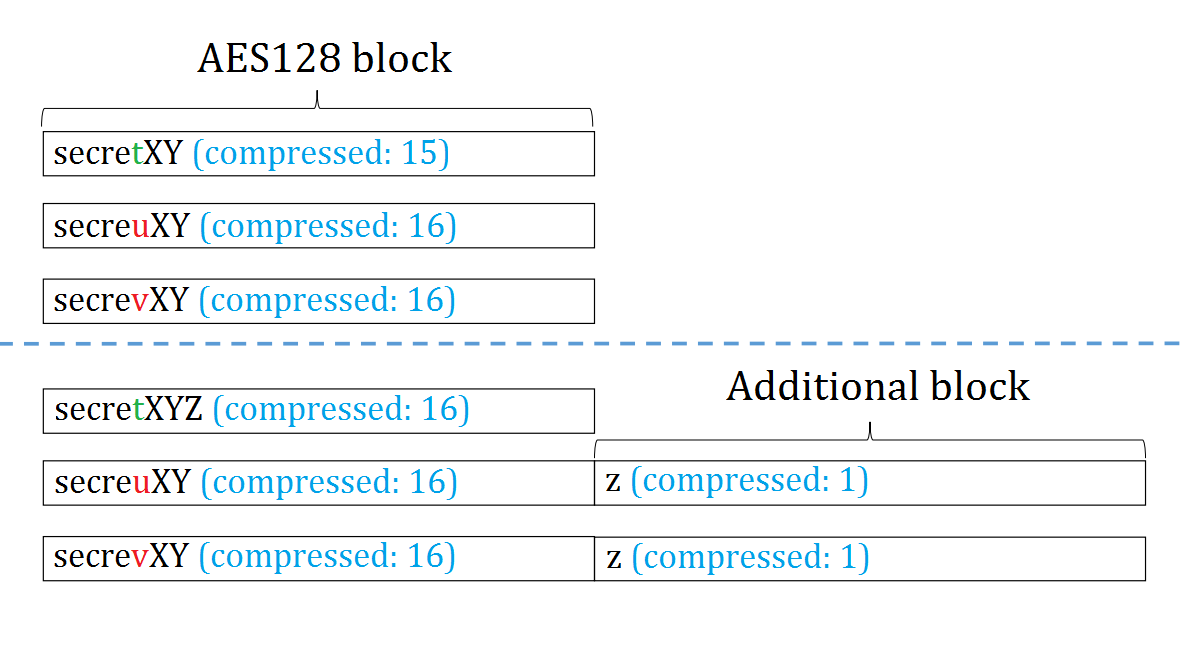
\includegraphics[width=0.48\textwidth]{figures/block_alignment.png}
      \caption{The block alignment method}
      \label{fig:block_alignment}
   \end{figure}

\subsubsection{Reflection computation methods}\label{subsec:reflectionmethods}
So far we have described the need for building and analysing reflections to
distinguish a single candidate in the secret's alphabet $\Sigma$ as the correct
one. In this section, we present two methods for constructing the reflections.

The first method is serial construction described in section
\ref{subsec:rupture_attack_design}. The complexity of this method is
$\mathcal{O}(|\Sigma|)$ and the round ends by finding a character of the secret.

The second method of attack is divide and conquer. The alphabet is now divided
into two subsets $\Sigma_1$ and $\Sigma_2 = \Sigma \setminus \Sigma_1$, where
$|\Sigma_1| = |\Sigma_2| = \ceil{|\Sigma| / 2}$. The reflection string for
$\Sigma_1$ consists of $|\Sigma_1|$ substrings separated by an annotation symbol
$\beta$. Each substring is built by concatenating the known prefix with a
candidate in $\Sigma_1$. For example, if $\Sigma_1$ is $\{``1", ``2"\}$ and the
known prefix is ``abc", using ``-" as $\beta$ the reflection is ``abc1-abc2".
The reflection string for $\Sigma_2$ is constructed similarly.

The end of each round marks the choice of subset $\Sigma_i$ that contains the
correct alphabet symbol. Each round reduces the alphabet by half, so the
complexity of this method is $\mathcal{O}(log|\Sigma|)$. When $|\Sigma_i| = 1$
the attack stage is completed and a character of the secret is decrypted.
Figure \ref{fig:divide_and_conquer} depicts the reflection sequence for the case
when the $\Sigma$ is the set of digits.

   \begin{figure}[thpb]
      \centering
          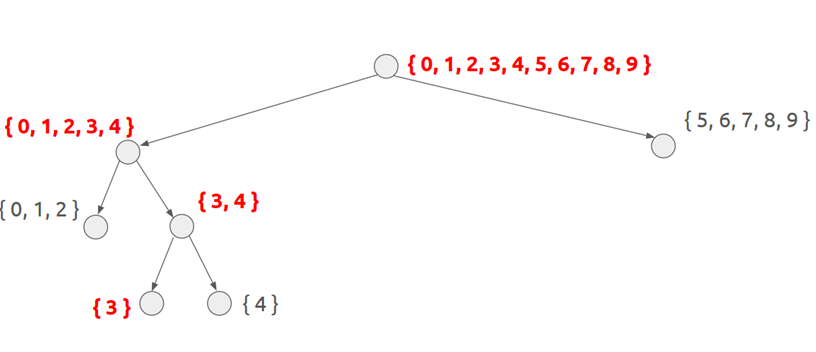
\includegraphics[width=0.48\textwidth]{figures/divide_and_conquer.png}
      \caption{The divide \& conquer method}
      \label{fig:divide_and_conquer}
   \end{figure}

\subsubsection{Request parallelization}\label{subsec:parallel}
Modern web servers are able to handle multiple parallel requests and
browsers can issue a certain amount of parallel requests per domain. This
functionality enables the adversary to issue multiple parallel requests per
candidate and efficiently reduce the execution time of the attack.

\subsubsection{Request soup}
Previous sections demonstrated the need for multiple requests per reflection
string $r_i$. However, communication is time expensive, so in many cases it is
preferable to issue multiple requests for a candidate and treat them as a set
rather than separately. This is the case for BREACH, where a set consists of
requests for a candidate $s_i$ in alphabet $\Sigma$. Bigger request sets result
in less time delay and the adversary can use the mean length over the number of
requests in the set without caring for each individual request's length.
